%!TEX root = ../main.tex
\section{Interface}
Interfacet som befinder sig på systemet, kan som udgangspunkt ligne skitsen som ses her på figur \ref{fig:Interface1}. Dette Interface skal befinde sig på en touchskærm.

\begin{figure}[ht]
	\centering
	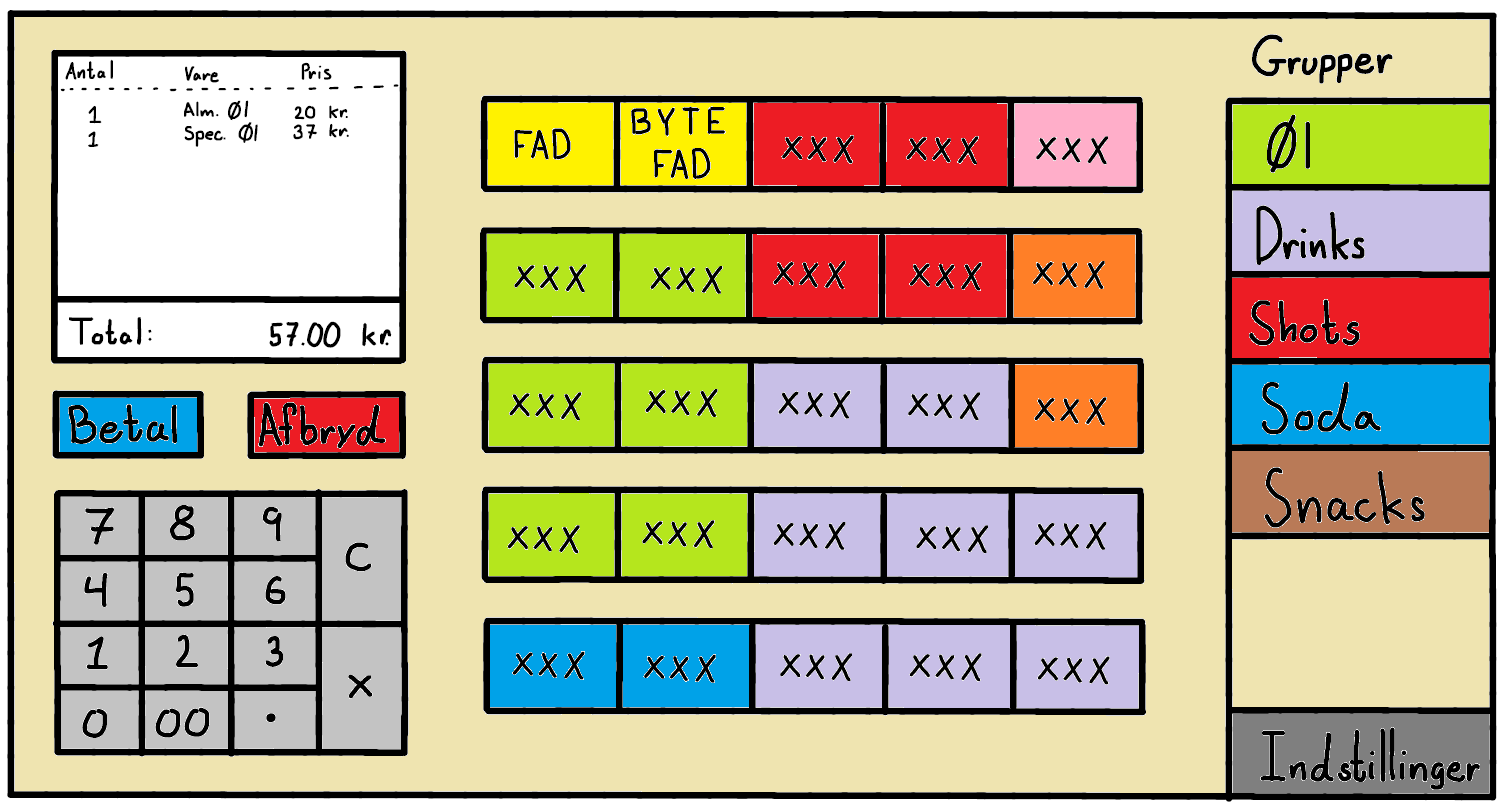
\includegraphics[width=0.8\textwidth]{Kravspecifikation/Interface/Interface1F.png}
	\caption{Skitse for Bruger interface på systemet - grupper}
	\label{fig:Interface1}
\end{figure}

For at give Bartenderen mulighed for at udføre en hurtig betjening, skal alle valg kunne tages på samme skærmbillede, dette er mulig under fanen grupper, som ses på figur \ref{fig:Interface1}. 
\newline\newline
På skærmen kan bartenderen se en knap til hver vare, det kunne f.eks. være ''FAD'' for fadøl. Når bartenderen trykker på en vare vil den tilføjes varelisten og den totale pris vil blive opdateret. 

\begin{figure}[H]
	\centering
	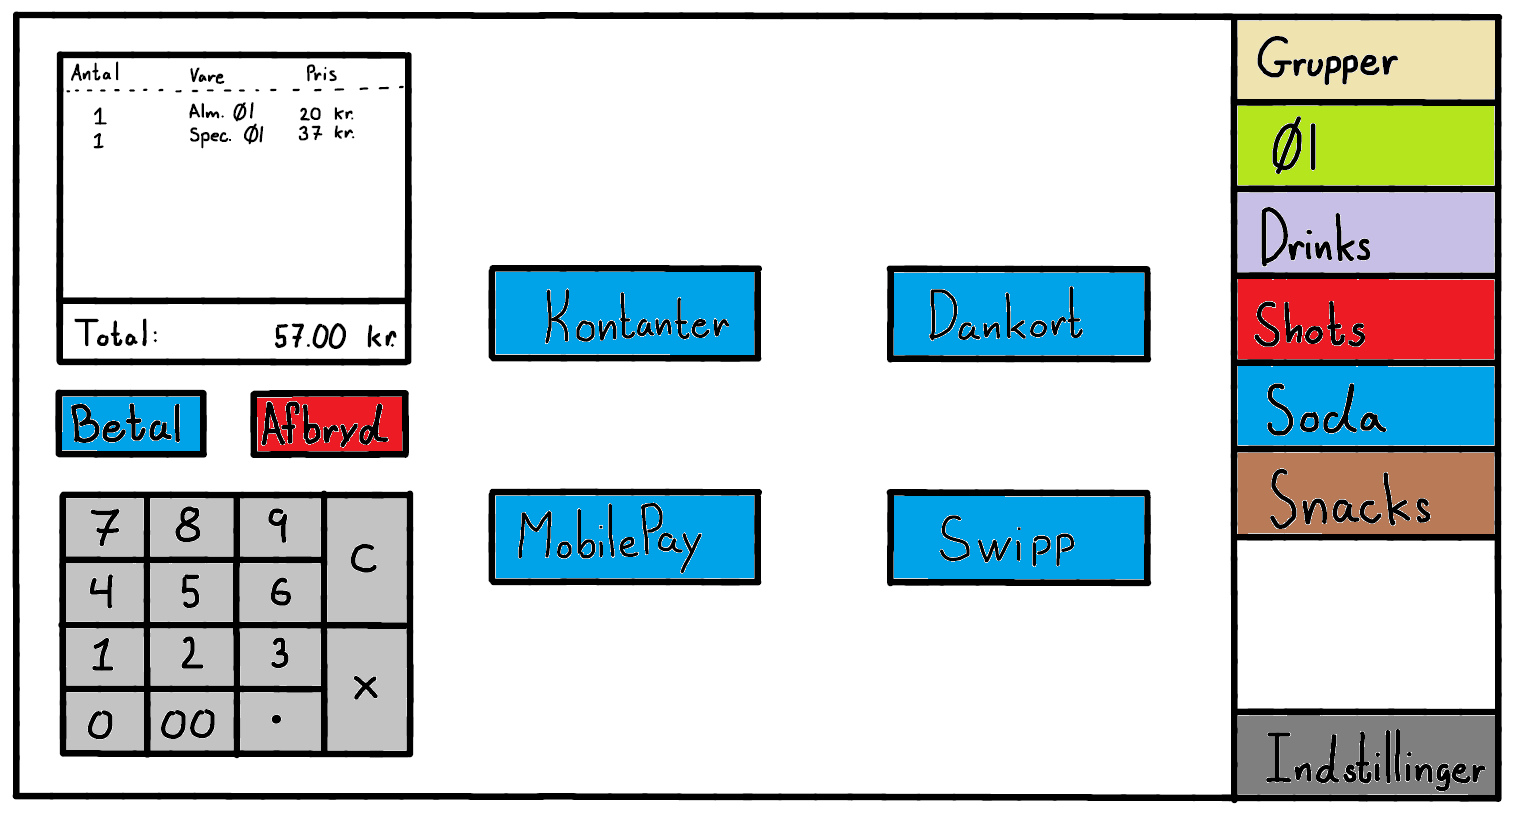
\includegraphics[width=0.8\textwidth]{Kravspecifikation/Interface/Interface3F.png}
	\caption{Skitse for Brugerinterface på systemet - betaling}
	\label{fig:Interface3}
\end{figure}
Når købet er slut kan Bartenderen trykke på betalingsknappen som tilgår det skærmbillede, med betalingsmulighederne, som ses på figur \ref{fig:Interface3}. Her trykker Bartenderen på den betalingsform der ønskes betales med. 
\newpage
I tilfælde af at Bartenderen ønsker noget mere præcis data om salget, f.eks. på dage hvor der ikke er så travlt, kan Bartenderen vælge at taste den specifikke vare ind, som kan findes under de forskellige faner ude i højre side af interfacet. Et eksempel på dette kunne f.eks. være ''Øl'', som ses på figur \ref{fig:Interface2}

\begin{figure}[ht]
	\centering
	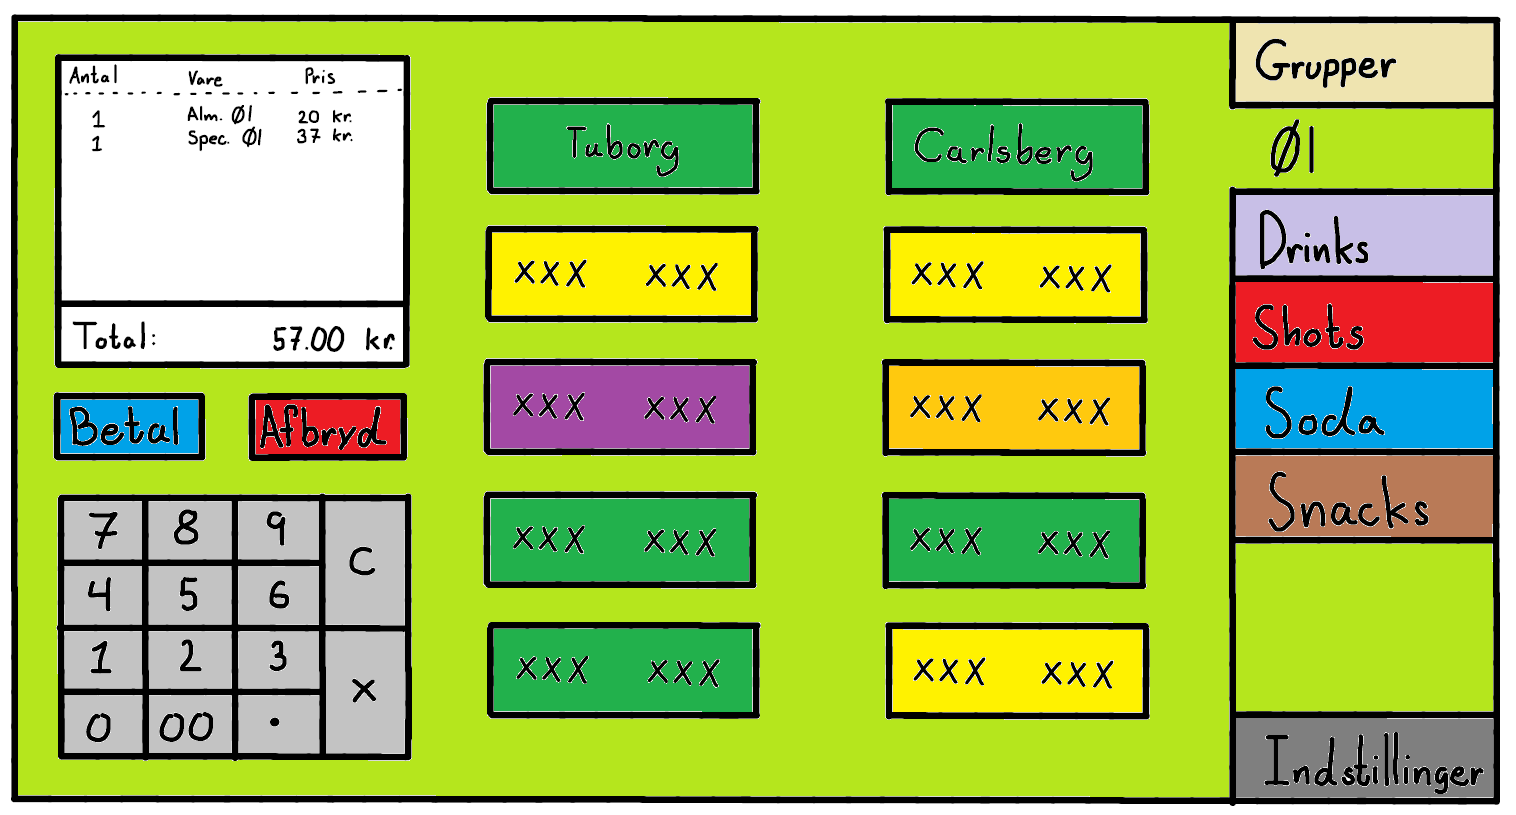
\includegraphics[width=0.8\textwidth]{Kravspecifikation/Interface/Interface2F.png}
	\caption{Skitse for Brugerinterface på kasseapparetet - Øl}
	\label{fig:Interface2}
\end{figure}

Her kan bartenderen så vælge en specifik øl, som f.eks. Tuborg, i stedet for at indtaste alm. øl eller en special øl.

